%!TEX program = xelatex
%%%%%%%%%%%%%%%%%%%%%%%这是导言部分的开始%%%%%%%%

%========= 导言部分声明文档的类型=================
\documentclass{article}

	%=========导言部分可可以加载宏包=================
	\usepackage{amsmath}                % 数学公式排版宏包
	\usepackage{amssymb}                % 数学符号命令宏包
	\usepackage{amsthm}                 % 数学定理宏包
	\usepackage[UTF8]{ctex}             % 中文输入宏包
	\usepackage[a4paper]{geometry}      % 页面设置宏包
	\usepackage{setspace}               % 行间距宏包
	\usepackage{graphicx}               % 图片宏包
	\usepackage{listings}               % 代码宏包
	\usepackage{color}					% 颜色宏包
	\usepackage{xcolor}                 % 颜色处理宏包
	\usepackage{float}                  % 浮动对象式样宏包
	\usepackage{fontspec}
	\usepackage{enumerate}				% 列举编号包
	
	%=========页面设置==============================
	\geometry{left=1cm,right=1cm,top=1cm,bottom=2cm}
	\onehalfspacing
	\setlength\parindent{0em}

	%=========代码格式设置============================
	\definecolor{dkgreen}{rgb}{0,0.6,0}
	\definecolor{gray}{rgb}{0.5,0.5,0.5}
	\definecolor{mauve}{rgb}{0.58,0,0.82}
	% \setmonofont{Consolas}
	\lstset{
		numbers = left, 	
		numberstyle = \color{gray}, 
		keywordstyle = \color{blue},
		commentstyle = \color{dkgreen}, 
		stringstyle = \color{mauve},
		basicstyle = \ttfamily,
		breaklines = true,
		frame = shadowbox, % 阴影效果
		rulesepcolor = \color{ red!20!green!20!blue!20} ,
		escapeinside = ``, % 英文分号中可写入中文
		xleftmargin = 2em,xrightmargin=2em, aboveskip=1em,
		framexleftmargin = 2em
	} 

%=========导言部分可以定义标题信息===============
\title{组会报告}
\author{徐益}
\date{\today}

%%%%%%%%%%%%%%%%%%%%%%%这是导言部分的结束%%%%%%%%%

%%%%%%%%%%%%%%%%%%%%%%%这是正文部分的开始%%%%%%%%%
\begin{document}

%=========生成标题================================
\maketitle

%=========开始正文的输入==========================

%===========第一节=================
\section{工作内容}

1. 更新DPDK

2. 学习LDPC相关内容及编码部分代码

%===========第一节=================
\section{更新DPDK18.05}

\begin{figure}[H]
	\centering
	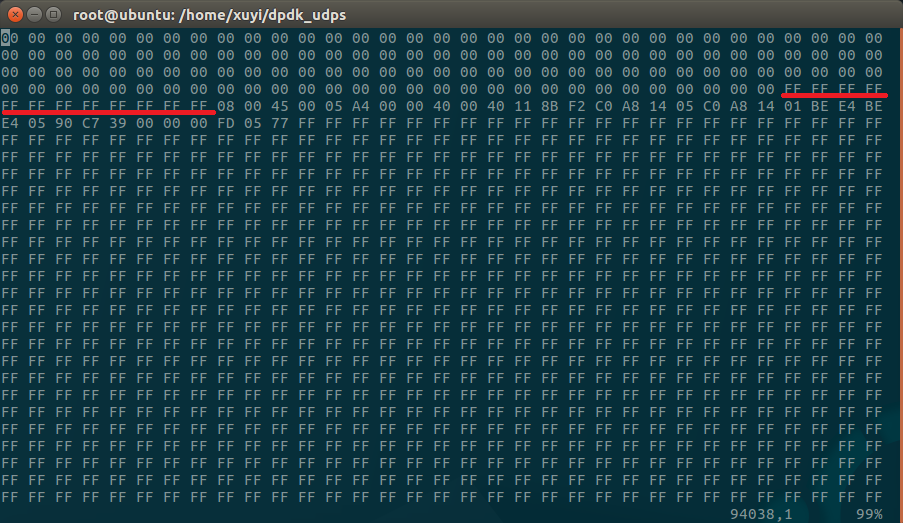
\includegraphics[width = \textwidth]{token_tc_bug.png}
	\caption{更新后仍存在内存覆盖、丢包问题}
\end{figure}

%===========第二节=================
\section{LDPC相关内容及编码部分代码学习}
\subsection{校验矩阵的构造}
\subsubsection{随机构造法}
\begin{enumerate}
	\item Gallager构造法
	\item 旋转矩阵构造法
	\item PEG构造法
\end{enumerate}
\subsubsection{结构化构造法}
\begin{enumerate}[--]
	\item 准循环(Quasi-Cyclic)构造法
\end{enumerate}
A QC-LDPC code is given by the null space of an array of sparse circulants of 
the same size. For two positive integers $c$ and $t$ with $c\leq t$, consider the 
folowing $c\times t$ array of $b\times b$ circulants over GF(2):
\begin{equation}
	\textbf{H}_{qc}=\begin{bmatrix}
		\textbf{A}_{1,1}&\textbf{A}_{1,2}&\cdots&\textbf{A}_{1,t}\\
		\textbf{A}_{2,1}&\textbf{A}_{2,2}&\cdots&\textbf{A}_{2,t}\\
		\vdots&\vdots&\ddots&\vdots\\
		\textbf{A}_{c,1}&\textbf{A}_{c,2}&\cdots&\textbf{A}_{c,t}
	\end{bmatrix}
\end{equation}
\subsection{编码算法}
Let $\textbf{H}_{qc}=\begin{bmatrix}\textbf{H}_{1}&\textbf{H}_{2}\end{bmatrix}$ be 
the partitioned base parity check matrix, where $\textbf{H}_{1}$ is an $(N-M)\times
M$ matrix, and $\textbf{H}_{2}$ is an $(N-M)\times (N-M)$ matrix. Let $\textbf{c}=
\begin{bmatrix}\textbf{m}&\textbf{p}\end{bmatrix}$ be a codeword block, where 
$\textbf{m}$ and $\textbf{p}$ denote information and parity bit sequences, respectively. 
From the property that the correct codeword satisfies the parity check equation, the 
parity bit sequence $\textbf{p}$ can be derived as follows,
\begin{equation}
	\textbf{H}_{qc}\cdot \textbf{c}^ \mathrm{T}=\textbf{H}_1\cdot \textbf{m}^\mathrm{T}+
	\textbf{H}_2\cdot \textbf{p}^\mathrm{T}=0
\end{equation}
\begin{equation}
	\textbf{p}^\mathrm{T}=\textbf{H}_2^{-1}\cdot\textbf{H}_1\cdot \textbf{m}^\mathrm{T}
\end{equation}
Since $\textbf{H}_1$ is a sparse matrix, and $\textbf{H}_2^{-1}$ has a regular pattern, 
the matrix-vector multiplications of (3) have linear complexity.
\subsection{min-sum译码算法}
\begin{figure}[H]
	\centering
	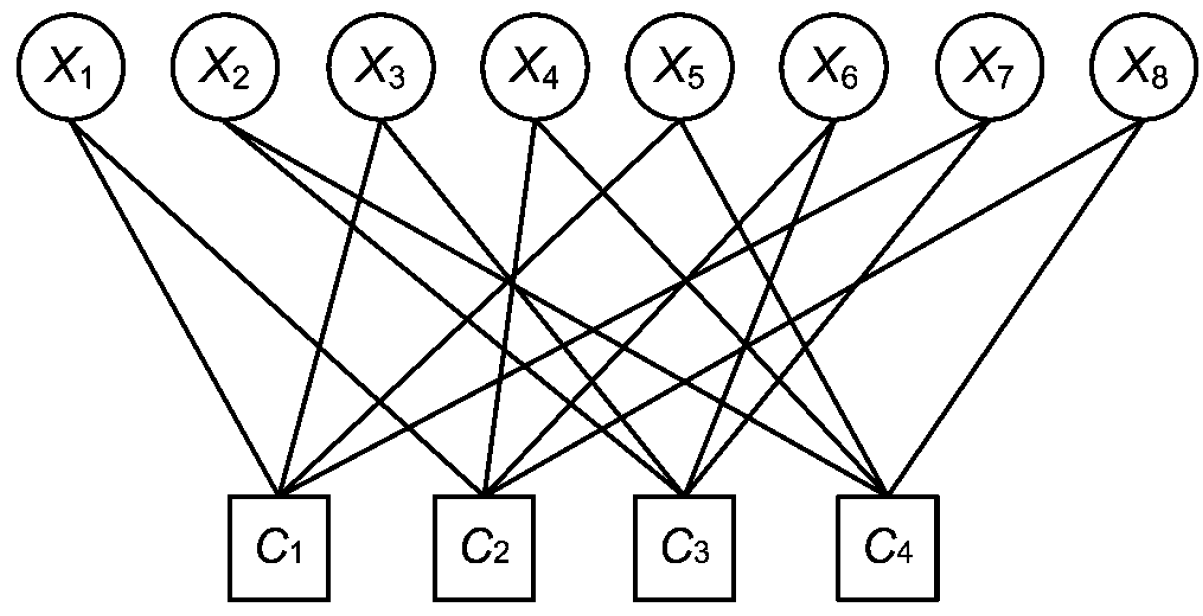
\includegraphics[width = .4\textwidth]{Tanner.png}
\end{figure}

1) Initialize the iteration counter, $i$, to 1 and let $I_M$ be the maximum number of 
iterations allowed.\\
2) Initialize $z^{(0)}_{mn}$ to the $a$ posteriori LLR, $\lambda _n=\log(P(v_n=0|y_n)/
P(v_n=1|y_n))$ for $1\leq n\leq N,m\in M(n)$.\\
3) Update the check nodes, i.e., for $1\leq m\leq M, n\in N(m)$, calculate:
\begin{equation}
	\epsilon^{(i)}_{mn}=\min_{n'\in N(m)\textbackslash n}|z^{(i)}_{mn'}|\prod_{n'\in 
	N(m)\textbackslash n}\mathrm {sgn}(z^{(i)}_{mn'}).
\end{equation}
4) Update the variable nodes, i.e., for $1\leq n \leq N,m\in M(n)$, calculate:
\begin{equation}
	z^{i}_{mn}=\sum_{m'\in M(n)\textbackslash m}\epsilon^{(i)}_{m'n}.
\end{equation}
5) Apply a hard decision, i.e., compute $\hat{W}=(\hat{w}_1,\hat{w}_2,...,\hat{w}_N)$
where element $\hat{w}_n=\left\{\begin{aligned}
	0, & \mathrm{if} \lambda _n+\sum\nolimits_{m\in M(n)}\epsilon^{(i)}_{mn}\geq 0, \\
	1, & \mathrm{otherwise}.\end{aligned}
	\right.$\\
If $\hat{W}H^T=0$ or $i\geq I_M$, stop decoding and go to step 6. Otherwise set 
$i=i+1$ and go to step 3.\\
6) Output $\hat{W}^{(i)}$ as the decoder output.

% \begin{figure}[H] 
% 	\flushleft
% 	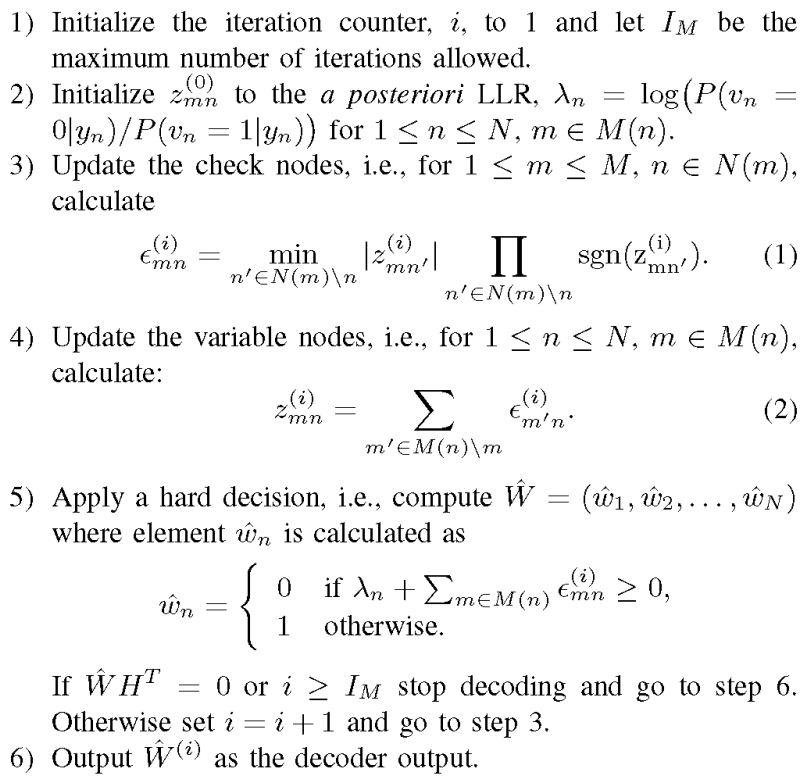
\includegraphics[width = .6\textwidth]{min-sum.png}
% \end{figure}

%===========第三节=================
% \section{修改流量控制方式}


%===========第四节=================
% \section{其他改进方向}
% 1. 选择更大的DPDK发送页。\\

% 2. 选择更优的流量控制策略。\\

%===========下周计划=================
\section{下阶段计划}
1. 完成LDPC译码matlab仿真\\
2. 尝试C语言实现

\end{document}
%%%%%%%%%%%%%%%%%%%%%%%这是正文部分的结束%%%%%%%%%%%%